\documentclass[
	letterpaper, % Paper size, specify a4paper (A4) or letterpaper (US letter)
	10pt, % Default font size, specify 10pt, 11pt or 12pt
]{CSUniSchoolLabReport}

%----------------------------------------------------------------------------------------
%	REPORT INFORMATION
%----------------------------------------------------------------------------------------

\title{Experiment Two\\ Fundamentals of Electromagnetics Lab \\ EECE2530/1} % Report title

\author{Michael \textsc{Brodskiy}\\ \small \href{mailto:Brodskiy.M@Northeastern.edu}{Brodskiy.M@Northeastern.edu}}

\date{October 11, 2023} % Date of the report

%----------------------------------------------------------------------------------------


\begin{document}

\maketitle % Insert the title, author and date using the information specified above

\begin{center}
	\begin{tabular}{l r}
		Date Performed: & October 4, 2023 \\ % Date the experiment was performed
        Partners: & Manas \textsc{Mahajan} \& Priyam \textsc{Modi} \\ % Partner names
		Instructor: & Professor \textsc{Marengo-Fuentes} \\ % Instructor/supervisor
        TAs: & Nicolas \textsc{Casilli} \& Farah \textsc{Ben Ayed} \\ % Teachers Assistants 
	\end{tabular}
\end{center}

\newpage

\begin{abstract}

  The goal of this laboratory experiment is to determine the dielectric constant of a coaxial cable by measuring the voltage standing wave ratio, as well as the lengths of lines at which the standing wave ratio minimums occur. To do this, the use of a signal generator connected to a slotted line, which, in turn, is connected to a standing wave ratio meter is employed.

\end{abstract}

\begin{flushleft}

  \textsc{Keywords:} \underline{dielectric constant}, \underline{coaxial}, \underline{voltage standing wave ratio}, \underline{signal generator}, \underline{slotted line}, \underline{standing wave ratio meter}

\end{flushleft}

\newpage

\section{Equipment}

\hspace{.5 in} Available equipment included:\\

\begin{itemize}

  \item Microwave Signal Generator

  \item Slotted Line (HP 809C)

  \item Voltage Standing Wave Ratio Meter (HP415E)

  \item Coaxial Cables

\end{itemize}

\section{Introduction \& Objectives}

First and foremost, we began by applying the correct settings to the signal generator — most importantly, a frequency of $2.3[\si{\giga\hertz}]$. Next, we calibrated the slotted line and voltage standing wave ratio (VSWR) meter without any components connected to the coaxial cable. \\

With all of our components ready and assembled, we measure $l_1$ and $l_2$, or the first two minima of the VSWR starting from the right. Then, we added a short cap with an RCL2 onto the slotted transmission line, after which we found the voltage minimum between $l_1$ and $l_2$, recording the readings as $S_{short}$ and $l_{short}$. Next, the cap was removed, yielding an open circuit, and the same steps were repeated to obtain $l_{open}$ and $S_{short}$.\\

With all of the necessary measurements, we then determine the value of the dielectric constant, $\varepsilon_r$, using the following flowchart shown in Figure \ref{fig:1}. These steps were then repeated for a wave of frequency $2.7[\si{\giga\hertz}]$.

\begin{figure}[H]
  \centering
  \tikzset{every picture/.style={line width=0.75pt}} %set default line width to 0.75pt        

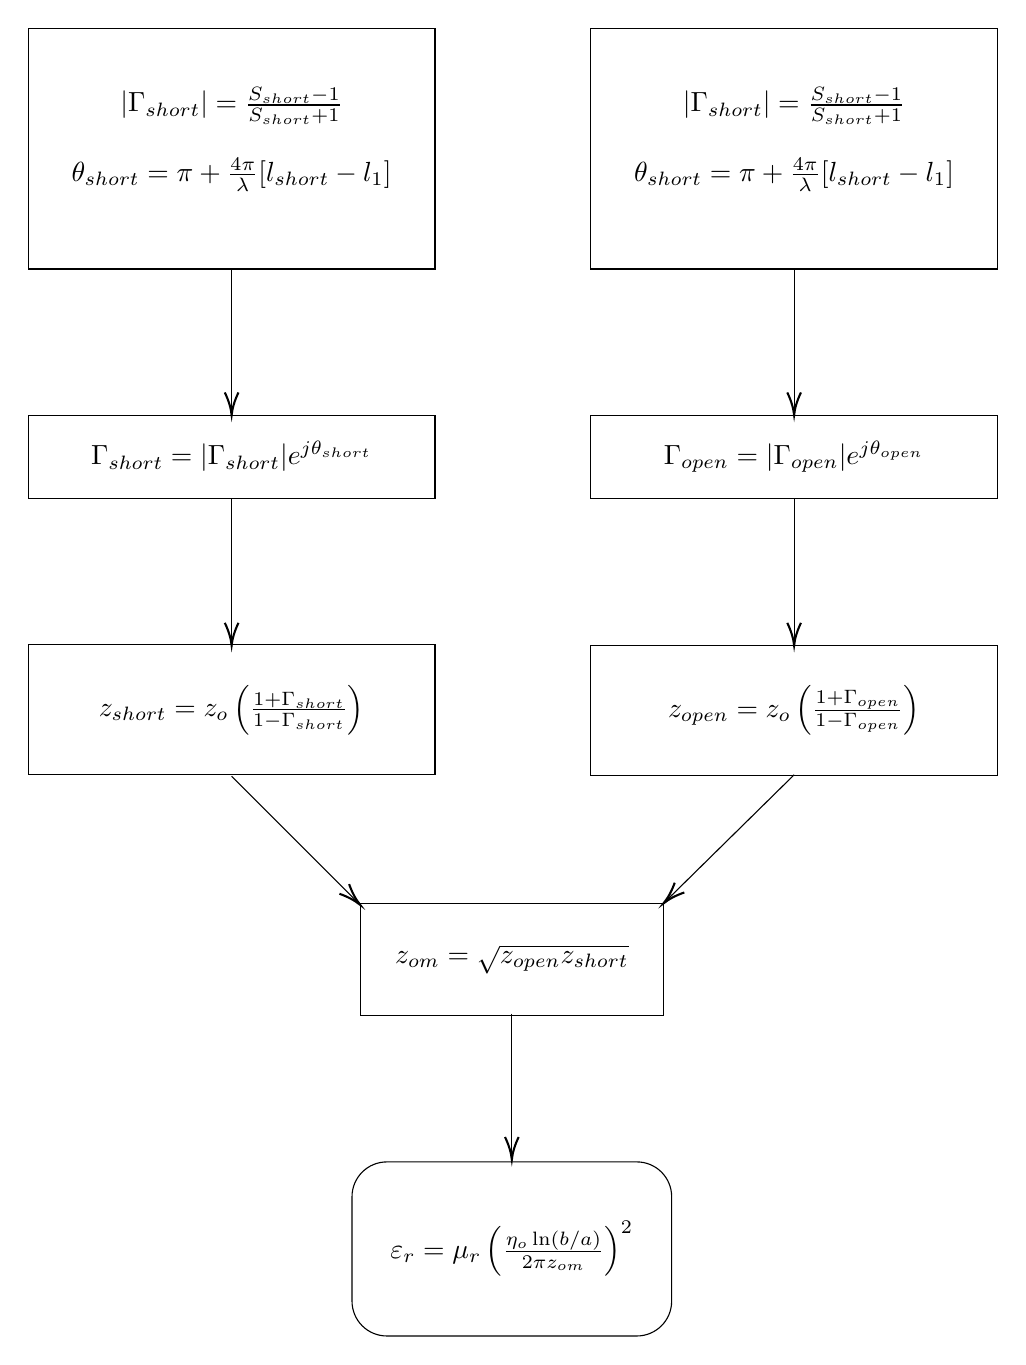
\begin{tikzpicture}[x=0.75pt,y=0.75pt,yscale=-1,xscale=1]
%uncomment if require: \path (0,657); %set diagram left start at 0, and has height of 657

%Shape: Rectangle [id:dp7126735491988057] 
\draw   (94,8) -- (290,8) -- (290,124) -- (94,124) -- cycle ;
%Shape: Rectangle [id:dp5768752679868709] 
\draw   (365,8) -- (561,8) -- (561,124) -- (365,124) -- cycle ;
%Straight Lines [id:da34420598529979385] 
\draw    (192,124) -- (192,192.42) ;
\draw [shift={(192,194.42)}, rotate = 270] [color={rgb, 255:red, 0; green, 0; blue, 0 }  ][line width=0.75]    (10.93,-3.29) .. controls (6.95,-1.4) and (3.31,-0.3) .. (0,0) .. controls (3.31,0.3) and (6.95,1.4) .. (10.93,3.29)   ;
%Straight Lines [id:da8417641803446987] 
\draw    (463,124) -- (463,192.42) ;
\draw [shift={(463,194.42)}, rotate = 270] [color={rgb, 255:red, 0; green, 0; blue, 0 }  ][line width=0.75]    (10.93,-3.29) .. controls (6.95,-1.4) and (3.31,-0.3) .. (0,0) .. controls (3.31,0.3) and (6.95,1.4) .. (10.93,3.29)   ;
%Shape: Rectangle [id:dp0887264533380483] 
\draw   (94,194.42) -- (290,194.42) -- (290,234.42) -- (94,234.42) -- cycle ;
%Shape: Rectangle [id:dp06732063654377773] 
\draw   (365,194.42) -- (561,194.42) -- (561,234.42) -- (365,234.42) -- cycle ;
%Straight Lines [id:da02670218063219898] 
\draw    (192,235) -- (192,303.42) ;
\draw [shift={(192,305.42)}, rotate = 270] [color={rgb, 255:red, 0; green, 0; blue, 0 }  ][line width=0.75]    (10.93,-3.29) .. controls (6.95,-1.4) and (3.31,-0.3) .. (0,0) .. controls (3.31,0.3) and (6.95,1.4) .. (10.93,3.29)   ;
%Straight Lines [id:da7673855623440871] 
\draw    (463,235) -- (463,303.42) ;
\draw [shift={(463,305.42)}, rotate = 270] [color={rgb, 255:red, 0; green, 0; blue, 0 }  ][line width=0.75]    (10.93,-3.29) .. controls (6.95,-1.4) and (3.31,-0.3) .. (0,0) .. controls (3.31,0.3) and (6.95,1.4) .. (10.93,3.29)   ;
%Shape: Rectangle [id:dp5668464351322218] 
\draw   (94,305.13) -- (290,305.13) -- (290,367.71) -- (94,367.71) -- cycle ;
%Shape: Rectangle [id:dp387927866207471] 
\draw   (365,305.42) -- (561,305.42) -- (561,368) -- (365,368) -- cycle ;
%Straight Lines [id:da24219615840965547] 
\draw    (463,367.71) -- (401.43,428.31) ;
\draw [shift={(400,429.71)}, rotate = 315.46] [color={rgb, 255:red, 0; green, 0; blue, 0 }  ][line width=0.75]    (10.93,-3.29) .. controls (6.95,-1.4) and (3.31,-0.3) .. (0,0) .. controls (3.31,0.3) and (6.95,1.4) .. (10.93,3.29)   ;
%Shape: Rectangle [id:dp3050012272660283] 
\draw   (254,429.71) -- (400,429.71) -- (400,483.71) -- (254,483.71) -- cycle ;
%Straight Lines [id:da5168465937110438] 
\draw    (192,368.42) -- (252.59,429.01) ;
\draw [shift={(254,430.42)}, rotate = 225] [color={rgb, 255:red, 0; green, 0; blue, 0 }  ][line width=0.75]    (10.93,-3.29) .. controls (6.95,-1.4) and (3.31,-0.3) .. (0,0) .. controls (3.31,0.3) and (6.95,1.4) .. (10.93,3.29)   ;
%Straight Lines [id:da14392593984104596] 
\draw    (327,482.71) -- (327,551.13) ;
\draw [shift={(327,553.13)}, rotate = 270] [color={rgb, 255:red, 0; green, 0; blue, 0 }  ][line width=0.75]    (10.93,-3.29) .. controls (6.95,-1.4) and (3.31,-0.3) .. (0,0) .. controls (3.31,0.3) and (6.95,1.4) .. (10.93,3.29)   ;
%Rounded Rect [id:dp28729239157386566] 
\draw   (250,570.97) .. controls (250,561.71) and (257.51,554.2) .. (266.77,554.2) -- (387.23,554.2) .. controls (396.49,554.2) and (404,561.71) .. (404,570.97) -- (404,621.29) .. controls (404,630.56) and (396.49,638.07) .. (387.23,638.07) -- (266.77,638.07) .. controls (257.51,638.07) and (250,630.56) .. (250,621.29) -- cycle ;

% Text Node
\draw (192,55.6) node [anchor=south] [inner sep=0.75pt]    {$|\Gamma _{short} |=\frac{S_{short} -1}{S_{short} +1}$};
% Text Node
\draw (192,69.4) node [anchor=north] [inner sep=0.75pt]    {$\theta _{short} =\pi +\frac{4\pi }{\lambda }[ l_{short} -l_{1}]$};
% Text Node
\draw (463,55.6) node [anchor=south] [inner sep=0.75pt]    {$|\Gamma _{short} |=\frac{S_{short} -1}{S_{short} +1}$};
% Text Node
\draw (463,69.4) node [anchor=north] [inner sep=0.75pt]    {$\theta _{short} =\pi +\frac{4\pi }{\lambda }[ l_{short} -l_{1}]$};
% Text Node
\draw (192,214.42) node    {$\Gamma _{short} =|\Gamma _{short} |e^{j\theta _{short}}$};
% Text Node
\draw (463,214.42) node    {$\Gamma _{open} =|\Gamma _{open} |e^{j\theta _{open}}$};
% Text Node
\draw (192,336.42) node    {$z_{short} =z_{o}\left(\frac{1+\Gamma _{short}}{1-\Gamma _{short}}\right)$};
% Text Node
\draw (463,336.71) node    {$z_{open} =z_{o}\left(\frac{1+\Gamma _{open}}{1-\Gamma _{open}}\right)$};
% Text Node
\draw (327,456.71) node    {$z_{om} =\sqrt{z_{open} z_{short}}$};
% Text Node
\draw (327,596.13) node    {$\varepsilon _{r} =\mu _{r}\left(\frac{\eta _{o}\ln( b/a)}{2\pi z_{om}}\right)^{2}$};


\end{tikzpicture}

  \caption{Flowchart for Calculations}
  \label{fig:1}
\end{figure}

\section{Results \& Analysis} 

We begin with the values we measured using the slotted line (length values in centimeters):

\begin{center}
\begin{tabular}[h!]{|c|c|c|c|c|c|c|c|c|}
  \hline
  $f\,[\si{\giga\hertz}]$ & $l_1$ & $l_2$ & $\lambda_{theor}$ & $\lambda_{exp}$ & $S_{short}$ & $l_{short}$ & $S_{open}$ & $l_{open}$\\
  \hline
  2.3 & 10.5 & 17.25 & 13.034 & 13.2 & 1.22 & 13.2 & 1.205 & 10.55\\
  \hline
  2.7 & 10.7 & 16.7 & 11.103 & 11.8 & 1.12 & 11.8 & 1.205 & 14.3\\
  \hline
\end{tabular}
\end{center}

Next, we calculate the magnitude of the reflection constant and phase angle for the two frequencies:

$$|\Gamma_{short,2.3}|=\frac{1.22-1}{1.22+1}=.099099$$
$$\theta_{short,2.3}=\pi+\frac{4\pi}{.132}\left[ .132-.105 \right]=5.712$$
$$|\Gamma_{open,2.3}|=\frac{1.205-1}{1.205+1}=.092971$$
$$\theta_{open,2.3}=\pi+\frac{4\pi}{.132}\left[ .1055-.105 \right]=3.1892$$

We now repeat for the 2.7 $[\si{\giga\hertz}]$ values:

$$|\Gamma_{short,2.7}|=\frac{1.12-1}{1.12+1}=.056604$$
$$\theta_{short,2.7}=\pi+\frac{4\pi}{.118}\left[ .118-.107\right]=4.313$$
$$|\Gamma_{open,2.7}|=\frac{1.205-1}{1.205+1}=.092971$$
$$\theta_{open,2.7}=\pi+\frac{4\pi}{.118}\left[ .143-.107 \right]=6.9754$$

Next, we find the full expression for $\Gamma$:

$$\Gamma_{short,2.3}=.099099e^{5.712j}=.083367-.053577j$$
$$\Gamma_{open,2.3}=.092971e^{3.1892j}=-.092865-.0044237j$$
$$\Gamma_{short,2.7}=.056604e^{4.313j}=-.022009-.05215j$$
$$\Gamma_{open,2.7}=.092971e^{6.9754j}=.071572+.059338j$$

Next, we use these values to find the impedances of such loads:

$$z_{short,2.3}=50\left( \frac{1+.083367-.053577j}{.9166+.053577j} \right)=55.8316-2.7611j[\si{\ohm}]$$
$$z_{open,2.3}=50\left(\frac{1-.092865-.0044237j}{1+.092865+.0044237j}\right)=41.5011-0.3704j[\si{\ohm}]$$
$$z_{short,2.7}=50\left( \frac{1-.022009-.05215j}{1+.022009+.05215j} \right)=47.5924-4.9798j[\si{\ohm}]$$
$$z_{open,2.7}=50\left( \frac{1+.071572+.059338j}{1-.071572-.059338j} \right)=57.2708+6.8559j[\si{\ohm}]$$

We know combine the complementary impedance values to find $z_{om}$:

$$z_{om,2.3}=\sqrt{(55.8316-2.7611j)(41.5011-.03704j)}=48.1502-1.2114j[\si{\ohm}]$$
$$z_{om,2.7}=\sqrt{(47.5924-4.9798j)(57.2708+6.8559j)}=52.5352+0.3911j[\si{\ohm}]$$

We now use these values in the following formula, with $\mu=1$, $\eta_o=120\pi$, and coaxial radius values of outer length $7[\si{\milli\meter}]$ and inner length $3[\si{\milli\meter}]$:

$$\varepsilon_r=\mu_r\left(  \frac{\eta_o\ln\left( \frac{b}{a} \right)}{2\pi z_{om}}\right)^2$$

$$\varepsilon_{r,2.3}=\left( \frac{120\pi\ln\left(\frac{7}{3}\right)}{2\pi(48.1502-1.2114j)} \right)^2=1.112638+.056021j$$
$$\varepsilon_{r,2.7}=\left( \frac{120\pi\ln\left(\frac{7}{3}\right)}{2\pi(52.5352+.3911j)} \right)^2=.936271-.013940j$$

Both of the real part values are near 1, as expected for air.

\section{Conclusion}

\subsection{Questions}

\begin{enumerate}

  \item Compare values of $\varepsilon_r$ for the two frequencies and explain any differences. Should the values be the same? If not, what does it mean?

    We can see that the magnitudes of the two values differ by about 17.32\%. This is most likely because slight imprecisions in measurements have a significant effect on the result. Thus, we most likely measured the values involved with $2.3[\si{\giga\hertz}]$ to be slightly larger than their actual values, while the values associated with $2.7[\si{\giga\hertz}]$ were probably measured as smaller than their true values.\\

    We know the values should be the same, as the same coaxial cable would have the same dielectric constant, no matter the frequency (which explains why it is called the dielectric \underline{constant}). Given the age of the equipment used, it isn't too surprising that the values weren't measured as accurately as they could have been. 

  \item Which constraints should you take into account when choosing a transmission line?

    The most important constraints to consider are the dielectric constant and the magnetic permeability. Given that these properties can change the way electricity, and, thus, light travels within the transmission line, it is important to consider the effects of these before choosing transmission lines. Furthermore, the conductance, resistance, inductance, and capacitance of a line should always be considered. Since these factors depend on the length, the length should also be taken into account.

  \item Briefly explain 2 applications on which transmission lines are used

    One application in which transmission lines are used is cable television. Another application is the use of telegraph lines (thus the name telegrapher's equations). The transmission lines work by passing high-frequency signals. These signals can not be used with regular power lines since the energy loss becomes too great. Thus, regular cables lose power, and become lossy.

\end{enumerate}

\subsection{Summary}

Overall, given our measurements and calculations, we can see that the dielectric constant is just above 1 (approximately 1.03). This makes sense, as air would not make the ability of a charge to align with the polarity of a field more or less likely.

\end{document}
